\section{Shiloh, Philistia, and the Ascent to Zion}\label{sec:captivity-hiddenness-zion}

When Joshua had divided the inheritance of the tribes and the land rested from war, all Israel gathered in the central highlands of Ephraim and set up the tabernacle of the testimony at Shiloh (Jos 18:1). For generations the Ark of the Covenant rested there beneath curtains, far from the desert march and the camps of conquest. Yet the darkest hour of the Ark's history did not fall in the wastes of Sinai or before Canaanite chariots; it fell when Israel's own priests forgot the fear of the Lord and carried the throne of the Holy One onto a battlefield as though God could be commandeered like a charm. Between the emptied sanctuary of Shiloh and the joyful tent David pitched on Mount Zion stretches a long school of reverence---through captivity in Philistia, sudden judgment at Beth-shemesh, twenty quiet years on a hill in Judah, the stroke at Nachon's threshing floor, and three months of blessing under the roof of Obed-edom.

\subsection{Shiloh, Bethel, and the Tragedy of Presumption}

During the unsettled generations of the Judges, the Ark remained the single center of Israel's covenant assembly, though the sacred text records one solemn moment when the tribes gathered before it amid civil war against Benjamin. After suffering two shattering defeats, all the children of Israel came to the house of God, sat weeping before the Lord, fasted until evening, offered holocausts and peace offerings, and inquired of God while Phinehas, the son of Eleazar and grandson of Aaron, stood in ministry over the house (Judg 20:26--28). Here the ancient biblical versions preserve a revealing geographical divergence. At Judges 20:18 the Clementine Vulgate renders the Hebrew \textit{Beth-El} (literally ``house of God'') as \textit{in domum Dei, hoc est, in Silo}, which the Douay-Rheims translates ``the house of God, that is, to Silo,'' so that when Judges 20:26--27 returns to ``the house of God'' and declares, ``At that time the ark of the covenant of the Lord was there,'' the Latin text holds the Ark fixed at Shiloh. By contrast, the Greek Septuagint (rendered by Brenton as ``Baethel'') and English versions resting on the Masoretic Hebrew (such as the World English Bible and the Revised Version) take the name in both 20:18 and 20:26 as the town of \textbf{Bethel}, indicating that during the crisis of the Benjaminite war the Ark was brought south temporarily to Bethel for solemn inquiry near the field of battle before returning to its highland sanctuary at Shiloh.

By the opening of the First Book of Samuel (First Kings in the Vulgate and Douay-Rheims), Shiloh stands unmistakably as Israel's regular house of pilgrimage and sacrifice. Year by year Elkanah went up from his city upon the appointed days ``to adore and to offer sacrifice to the Lord of hosts in Silo'' (1 Sam 1:3). The wilderness tent had acquired fixed doorposts and a permanent threshold; the aged priest Eli sat upon his stool ``before the door of the temple of the Lord'' (\textit{ante postes templi Domini}, 1 Sam 1:9) while Hannah poured out her silent grief and prayed for a son. Inside that sanctuary unfolds one of the stillest scenes in all the Old Testament:

\begin{scriptureblock}
Before the lamp of God went out, Samuel slept in the temple of the Lord, where the ark of God was. \textnormal{(1 Sam 3:3)}
\end{scriptureblock}

The contrast drawn across the opening chapters of 1 Samuel is piercing. In the quiet before dawn, while the sanctuary lamp still burns, a docile boy sleeps beside the Ark and receives the word of the Lord with immediate obedience. Outside, however, Eli's sons Hophni and Phinehas serve as priests of the Lord in Shiloh (1 Sam 1:3) while despising the offerings and defiling the threshold of the tent. Nearness to the Ark does not shield unrepentant ministers: the very night Samuel hears God's voice beside the chest, the Lord pronounces irrevocable judgment upon Eli's house.

That judgment broke at Aphek and Ebenezer. Defeated in a first clash with the Philistines, the elders of Israel returned to camp and spoke words that lay bare the hollowness of their trust:

\begin{scriptureblock}
Why hath the Lord defeated us to day before the Philistines? Let us fetch unto us the ark of the covenant of the Lord from Silo, and let it come in the midst of us, that it may save us from the hand of our enemies. \textnormal{(1 Sam 4:3)}
\end{scriptureblock}

There is no fast, no repentance, no inquiry of the prophet Samuel. The elders speak of the Ark with a chilling neuter expectation---``that it may save us''---treating the covenant throne as a battlefield talisman that can force God's hand while His commandments are broken. Yet the sacred narrator pauses to state the true majesty of what they treated so casually: they sent to Shiloh and fetched ``the ark of the covenant of the Lord of hosts, sitting upon the cherubims,'' accompanied by the two corrupt priests Hophni and Phinehas (1 Sam 4:4). When the Ark entered the camp, ``all Israel shouted with a great shout, and the earth rang again'' (1 Sam 4:5). Hearing the roar and learning that the Ark of the Lord had arrived, even the Philistines trembled and sighed, ``God is come into the camp,'' recalling the plagues that had struck Egypt in the desert (1 Sam 4:6--8).

Yet the Philistines rallied one another to fight like men, and the Lord refused to lend His glory to presumption. Israel broke in disaster; ``there fell of Israel thirty thousand footmen. And the ark of God was taken: and the two sons of Heli, Ophni and Phinees, were slain'' (1 Sam 4:10--11). When a runner brought the news to Shiloh, ninety-eight-year-old Eli fell backward from his seat and died at the tidings that the Ark of God had been captured (1 Sam 4:18). At the same hour, the wife of Phinehas entered sudden labor and, dying, turned away from the women who announced the birth of a son, naming the child \textit{Ichabod}---``Where is the glory?'' or ``No glory'':

\begin{scriptureblock}
And she called the child Ichabod, saying: The glory is gone from Israel, because the ark of God was taken, and for her father in law, and for her husband: And she said: The glory is departed from Israel, because the ark of God was taken. \textnormal{(1 Sam 4:21--22)}
\end{scriptureblock}

\subsection{Exile in Philistia and Hiddenness at Kiriath-jearim}

To earthly eyes, the God of Israel seemed vanquished alongside His army. Bearing the Ark in triumph from Ebenezer---``the Stone of help'' (\textit{a lapide Adjutorii})---into Ashdod (\textit{Azotus}), the Philistines carried it into the temple of Dagon and set it beside their idol, as ancient conquerors displayed captive gods at the feet of their own deity (1 Sam 5:1--2). What happened in the darkness of that pagan shrine shattered every illusion of captivity. Israel could lose a battle; the Lord enthroned upon the cherubim could never be conquered.

When the men of Ashdod rose early the next morning, ``behold Dagon lay upon his face on the ground before the ark of the Lord'' (1 Sam 5:3). Supposing the fall an accident, the priests lifted their god and set him back in his place. The second morning brought decisive judgment:

\begin{scriptureblock}
And the next day again, when they rose in the morning, they found Dagon lying upon his face on the earth before the ark of the Lord: and the head of Dagon, and both the palms of his hands, were cut off upon the threshold: And only the stump of Dagon remained in its place. \textnormal{(1 Sam 5:4--5)}
\end{scriptureblock}

Without a single Israelite sword drawn, the Ark broke the idol from within its own shrine. Stripped of head and hands---deprived of counsel and stripped of power---the image of Dagon lay prostrate in involuntary homage across its own doorway, so that neither Dagon's priests nor any who entered his house trod upon that threshold thereafter (1 Sam 5:5). Nor did the judgment end with carved stone. The hand of the Lord weighed heavily upon Ashdod and its borders with painful tumors (``emerods'') and a plague of mice swarming out of the fields, until the citizens cried out: ``The ark of the God of Israel shall not stay with us: for his hand is heavy upon us, and upon Dagon, our god'' (1 Sam 5:6--7).

For seven months the Ark moved across the Philistine plain like an unconquerable king passing through rebel territory (1 Sam 6:1). Assembling in council, the lords of the Philistines sent the Ark inland to Gath (\textit{Geth}), where the same deadly slaughter and affliction fell upon small and great alike (1 Sam 5:8--9). From Gath they dispatched it to Ekron (\textit{Accaron}), whose inhabitants cried out at its approach: ``They have brought the ark of the God of Israel to us, to kill us and our people'' (1 Sam 5:10). Here an exact textual comparison across the ancient versions merits notice: whereas the Clementine Vulgate, Douay-Rheims, and Masoretic Hebrew tradition send the Ark from Gath to \textbf{Ekron} (\textit{Accaron}) at 1 Sam 5:10 and return the five Philistine lords to Ekron at 1 Sam 6:16, the Greek Septuagint (in Brenton's translation) sends the Ark to \textbf{Ashkelon} (\textit{Ascalon}) in 5:10 and sends the five lords back to Ashkelon in 6:16, even while still enumerating all five Philistine lordships---Ashdod, Gaza, Ashkelon, Gath, and Ekron---in the tally of the five golden trespass-offerings at 6:17. Across the entire pentapolis, the fear of death gripped every town and the cry of every city rose to heaven until the lords resolved to send the Ark back to its own place (1 Sam 5:11--12).

Even in parting, the Philistine priests and diviners read the lessons of sacred history more clearly than Israel's elders had done at Aphek. ``Why do you harden your hearts, as Egypt and Pharao hardened their hearts?'' they asked the lords, warning them not to send the Ark away empty but to render a golden guilt-offering of five tumors and five mice according to the five provinces, ``and you shall give glory to the God of Israel'' (1 Sam 6:3--6). To test whether the plague was truly the hand of Israel's God or mere chance, they fashioned ``a new cart: and two kine that have calved, on which there hath come no yoke,'' yoked the untrained milk cows to the cart carrying the Ark and the coffer of gold, and shut their nursing calves behind them at home (1 Sam 6:7--11).

Creation itself obeyed its Lord. Pulling straight away from their newborn calves against every pull of maternal instinct, ``the kine took the straight way, that leadeth to Bethsames, and they went along the way, lowing as they went: and turned not aside neither to the right hand nor to the left'' (1 Sam 6:12). The five lords of the Philistines walked behind in stunned silence as far as the border. Down in the valley, the men of Beth-shemesh (\textit{Bethsames}) were reaping wheat; ``and lifting up their eyes, they saw the ark, and rejoiced to see it'' (1 Sam 6:13). When the cart stopped beside a great stone in the field of Joshua the Beth-shemite, the Levites lifted down the Ark and the golden coffer onto the rock, split the timbers of the cart for firewood, and offered the two cows in holocaust to the Lord (1 Sam 6:14--15).

Yet the homecoming at Beth-shemesh turned swiftly from harvest joy to terror when irreverent curiosity profaned the sacred chest:

\begin{scriptureblock}
But he slew of the men of Bethsames, because they had seen the ark of the Lord, and he slew of the people seventy men, and fifty thousand of the common people. And the people lamented, because the Lord had smitten the people with a great slaughter. \textnormal{(1 Sam 6:19)}
\end{scriptureblock}

The double figure preserved in this verse---``seventy men, and fifty thousand of the common people'' (\textit{septuaginta viros, et quinquaginta millia plebis} in the Clementine Vulgate, with both numerals likewise present in the Septuagint and the Masoretic Hebrew)---has long stood as a famous textual difficulty, given the modest population of a Judean border town. Bishop Challoner, in his note on the verse, explains both that ``seen'' means having ``curiously looked into'' the Ark and that ``this plague reached to all the neighbouring country, as well as the city of Bethsames''; textual scholars have likewise noted the abrupt juxtaposition of seventy and fifty thousand in the received text. Leaving that manuscript crux honestly unresolved where the ancient versions stand in tension, the spiritual meaning of Beth-shemesh shines with unmistakable severity. Neither pagan captors nor Israelite reapers may peer casually into the dwelling of the Holy One. The shaken survivors voice the exact question of creaturely reverence: ``Who shall be able to stand before the Lord this holy God? and to whom shall he go up from us?'' (1 Sam 6:20).

Summoned down from the wooded hills above the valley, the men of \textbf{Kiriath-jearim} (\textit{Cariathiarim}, ``City of Forests'') came and brought the Ark up into Judah, ``and carried it into the house of Abinadab, in Gabaa: and they sanctified Eleazar, his son, to keep the ark of the Lord'' (1 Sam 7:1; as Challoner notes, \textit{in Gabaa} means ``on the hill''). There the Ark entered a long, hidden Sabbath of obscurity:

\begin{scriptureblock}
And it came to pass, that from the day the ark of the Lord abode in Cariathiarim, days were multiplied (for it was now the twentieth year) and all the house of Israel rested, following the Lord. \textnormal{(1 Sam 7:2)}
\end{scriptureblock}

The old sanctuary of Shiloh never received the Ark again. Through the long years of Samuel's ministry and the entire troubled reign of Saul, the Ark rested quietly inside a private household on a Judean hill---so far from the king's court that David would later tell all Israel, ``for we sought it not in the days of Saul'' (1 Chr 13:3). Guarded by the consecrated hands of Eleazar, the Ark waited in the hill country of Judah until Israel's repentance matured and David prepared its ascent to Mount Zion.

\subsection{Perez-Uzzah, Obed-edom, and the Ascent to Mount Zion}

When all twelve tribes gathered to anoint David king and his men captured the Jebusite stronghold of Jerusalem, David turned at once to the neglected heart of Israel's covenant worship (2 Sam [2 Kgs] 6:1--2; 1 Chr [1 Par] 13:1--6). Taking counsel with his captains of thousands and hundreds, he assembled Israel from Sihor of Egypt to the entrance of Hamath, gathering thirty thousand chosen men (seventy thousand in Brenton's Septuagint of 2 Sam 6:1), and rose up ``to fetch the ark of God, upon which the name of the Lord of Hosts is invoked, who sitteth over it upon the cherubims'' (2 Sam 6:2). At this verse a single Hebrew phrase (\textit{baale Yehudah}) yields an illuminating versional split: English translations following the Masoretic Hebrew (the World English Bible, Revised Version, and King James Version) take it as a place-name, ``from Baale Judah'' (an older name for Kiriath-jearim, matching 1 Chr 13:6, ``the hill of Cariathiarim which is in Juda''), whereas the Clementine Vulgate (\textit{de viris Juda}) and Douay-Rheims translate it of persons, ``of the men of Juda,'' and Brenton's Septuagint reads ``some of the rulers of Juda.''

Every outward sign of that first procession breathed festive energy. David and all Israel played before the Lord ``on all manner of instruments made of wood, on harps and lutes and timbrels and cornets and cymbals'' (2 Sam 6:5; 1 Chr 13:8). Yet enthusiasm had outrun obedience. In the wilderness, Moses had commanded that whenever the camp set forward, Aaron and his sons should shroud the Ark in the inner veil, violet skins, and a cloth of pure violet, and that only the consecrated Levites of the family of Kohath should bear it upon their shoulders by its staves, without ever touching the holy vessels ``lest they die'' (Num 4:5--6, 15; cf. Num 7:9, where Kohath received no ox-carts precisely because they bore the sanctuary upon their shoulders). Instead of keeping that plain ordinance, Israel copied the Philistine expedient of 1 Samuel 6 and loaded the Ark of God upon a new ox-cart driven by Abinadab's sons Uzzah (\textit{Oza}) and Ahio (2 Sam 6:3--4; 1 Chr 13:7).

When the cart reached the threshing floor of Nachon (called Chidon in 1 Chr 13:9), the oxen stumbled and made the Ark lean aside:

\begin{scriptureblock}
And when they came to the floor of Nachon, Oza put forth his hand to the ark of God, and took hold of it: because the oxen kicked and made it lean aside. And the indignation of the Lord was enkindled against Oza, and he struck him for his rashness: and he died there before the ark of God. \textnormal{(2 Sam 6:6--7)}
\end{scriptureblock}

Music died instantly upon the road. Troubled and grieved, David called that place ``The striking of Oza'' (\textit{Percussio Ozae}, 2 Sam 6:8; ``the Breach of Oza,'' 1 Chr 13:11; Hebrew \textit{Perez-Uzzah}). Sacred Scripture itself leaves no ambiguity regarding why the judgment fell. Preparing the second ascent, David summoned the priests Zadok and Abiathar and the heads of the Levitical houses and stated the exact law that had been broken: ``No one ought to carry the ark of God, but the Levites, whom the Lord hath chosen to carry it, and to minister unto himself for ever'' (1 Chr 15:2). Charging them to sanctify themselves, the king made open confession before all Israel:

\begin{scriptureblock}
Lest as the Lord at first struck us, because you were not present, the same should now also come to pass, by our doing some thing against the law. \textnormal{(1 Chr 15:13)}
\end{scriptureblock}

St. Robert Bellarmine, commenting on the awe owed to the Lord's earthly footstool in Psalm 131:8, draws Beth-shemesh and Uzzah together in a single austere warning: ``When the Bethsamites inspected the Ark with too much curiosity, over forty thousand of them were slain; and Oza, for merely touching it, was at once slain by God.'' Uzzah reached out not in hatred but in disregard of Numbers 4:15, where the Lord had forbidden even the sons of Kohath to touch the holy vessels lest they die; good intentions cannot supersede the order God Himself established for His sanctuary.

Standing in the stunned silence beside Nachon's threshing floor, King David voiced a trembling question that will echo across ten centuries into a quiet doorway in the Judean hills:

\begin{scriptureblock}
And David was afraid of the Lord that day, saying: How shall the ark of the Lord come to me? \textnormal{(2 Sam 6:9)}
\end{scriptureblock}

In the Clementine Vulgate the cry carries a spare, unforgettable gravity: \textit{Quomodo ingredietur ad me arca Domini?} (``How shall the ark of the Lord enter to me?''; echoed in 1 Chr 13:12, ``How can I bring in the ark of God to me?''). Refusing to bring the Ark into the city of David while Israel remained unprepared, the king turned it aside into the nearby household of \textbf{Obed-edom the Gittite} (\textit{Obededom Gethaei}, 2 Sam 6:10; whom 1 Chr 15:18, 21, 24 and 16:5 also rank among the Levitical gatekeepers and singers of the Ark). There the Ark remained for a quarter of a year:

\begin{scriptureblock}
And the ark of the Lord abode in the house of Obededom the Gethite three months: and the Lord blessed Obededom, and all his household. \textnormal{(2 Sam 6:11)}
\end{scriptureblock}

In the parallel notice of 1 Chronicles 13:14, the Clementine Vulgate crystallizes the scene in a Latin cadence that St. Luke will later reproduce almost word for word at the Visitation of the Blessed Virgin Mary: \textit{Mansit ergo arca Dei in domo Obededom tribus mensibus} (``And the ark of God remained in the house of Obededom three months''). Beneath a reverent roof, the very presence that had broken Dagon and struck down rash hands became pure blessing upon an entire household.

When word reached Jerusalem that the Lord had blessed Obed-edom and all his possessions because of the Ark, David returned with gladness---and this time with scrupulous obedience to Moses (2 Sam 6:12; 1 Chr 15:11--15). No cart rolled upon the road. Having sanctified themselves, ``the sons of Levi took the ark of God as Moses had commanded, according to the word of the Lord, upon their shoulders, with the staves'' (1 Chr 15:15). After the bearers had gone six paces, David sacrificed an ox and a ram (2 Sam 6:13; and when God helped the Levites carry the sacred burden, they offered seven oxen and seven rams, 1 Chr 15:26). Seven choirs marched with the king (2 Sam 6:12). Appointed under the chief singers Heman, Asaph, and Ethan, the Levitical musicians sounded cymbals of brass, psalteries, harps, and priestly trumpets ``that the joyful noise might resound on high'' (1 Chr 15:16, 19, 24, 28)---a solemn proclamation that Brenton's Septuagint renders ``to sound aloud with a voice of joy'' (1 Chr 15:16) and ``to lift up the voice'' (1 Chr 16:4).

Clothed in a robe of fine linen and girded with a priestly linen ephod (2 Sam 6:14; 1 Chr 15:27), David cast aside every reserve of royal self-importance. In the Douay-Rheims and Clementine Vulgate, ``David danced with all his might before the Lord'' (\textit{saltabat}, 2 Sam 6:14), and as all Israel brought the Ark into the city of David ``with joyful shouting, and with sound of trumpet'' (2 Sam 6:15), Saul's daughter Michal looked down through a window and ``saw king David leaping and dancing before the Lord: and she despised him in her heart'' (\textit{subsilientem atque saltantem}, 2 Sam 6:16; cf. 1 Chr 15:29, ``dancing and playing''). Notably, Brenton's Septuagint renders the verbs of 2 Samuel 6 with a musical emphasis rather than leaping, reading ``sounded with well-tuned instruments before the Lord'' at 2 Sam 6:14 and ``dancing and playing before the Lord'' at 2 Sam 6:16. Michal's disdain lays bare the permanent clash between worldly pride and liturgical adoration: she judged the king by the dignity of Saul's court, whereas David rejoiced as a servant before the King of glory.

At last the long pilgrimage from Shiloh crossed its royal threshold upon Mount Zion:

\begin{scriptureblock}
And they brought the ark of the Lord, and set it in its place in the midst of the tabernacle, which David had pitched for it: and David offered holocausts, and peace offerings before the Lord. \textnormal{(2 Sam 6:17)}
\end{scriptureblock}

Having offered holocausts and peace offerings, David blessed the people in the name of the Lord of hosts and distributed to every man and woman in Israel a loaf of bread, a portion of roasted beef, and fine flour fried with oil---a covenant banquet uniting king, priests, and people around the newly enthroned Ark (2 Sam 6:18--19; 1 Chr 16:1--3). Before that tent on Mount Zion he appointed Levites under Asaph, Zechariah, and Obed-edom himself ``to minister before the ark of the Lord, and to remember his works, and to glorify, and praise the Lord God of Israel'' (1 Chr 16:4--5).

\begin{threestable}{Station}{Scriptural Account}{Covenant Significance}
Shiloh (and Bethel) & Jos 18:1; Judg 20:18, 26--28; 1 Sam 1--4 & Highland sanctuary where Samuel hears God's call beside the Ark; profaned by Hophni and Phinehas and emptied when Israel treats the Ark as a battlefield charm.\\
\addlinespace[0.25em]
Philistine Pentapolis & 1 Sam 5:1--6:12 & Seven-month captivity in Ashdod, Gath, and Ekron (Ashkelon in LXX 5:10; 6:16); Dagon falls broken across his own threshold, proving the Lord is never conquered.\\
\addlinespace[0.25em]
Beth-shemesh & 1 Sam 6:13--21 & Two milk cows draw the Ark straight up from Philistia; joyful harvest welcome turns to dread when irreverent curiosity provokes divine judgment.\\
\addlinespace[0.25em]
Kiriath-jearim & 1 Sam 7:1--2; 1 Chr 13:3--6 & Twenty years of quiet custody in Abinadab's house on the hill under consecrated Eleazar, awaiting a king who will seek the Lord.\\
\addlinespace[0.25em]
Threshing Floor of Nachon & 2 Sam 6:3--9; 1 Chr 13:7--12; 15:2, 13 & Imitating the Philistine cart violates Numbers 4; Uzzah's death halts the march and draws from David the trembling cry, ``How shall the ark of the Lord come to me?''\\
\addlinespace[0.25em]
House of Obed-edom & 2 Sam 6:10--12; 1 Chr 13:13--14 & Three months of stillness (\textit{mansit ... tribus mensibus}) transform dread into abundant blessing upon an entire reverent household.\\
\addlinespace[0.25em]
Tent on Mount Zion & 2 Sam 6:12--19; 1 Chr 15:15--16:5 & Levitical shoulder-bearing, sacrifice every six paces, David's joyful dancing, covenant meal, and perpetual liturgy on the royal hill of Jerusalem.\\
\end{threestable}

\ifdefined\TriptychPrintEdition
\Needspace{30\baselineskip}
\begin{center}
\begin{tikzpicture}
  \node[anchor=south west, inner sep=0] (image) at (0,0) {%
    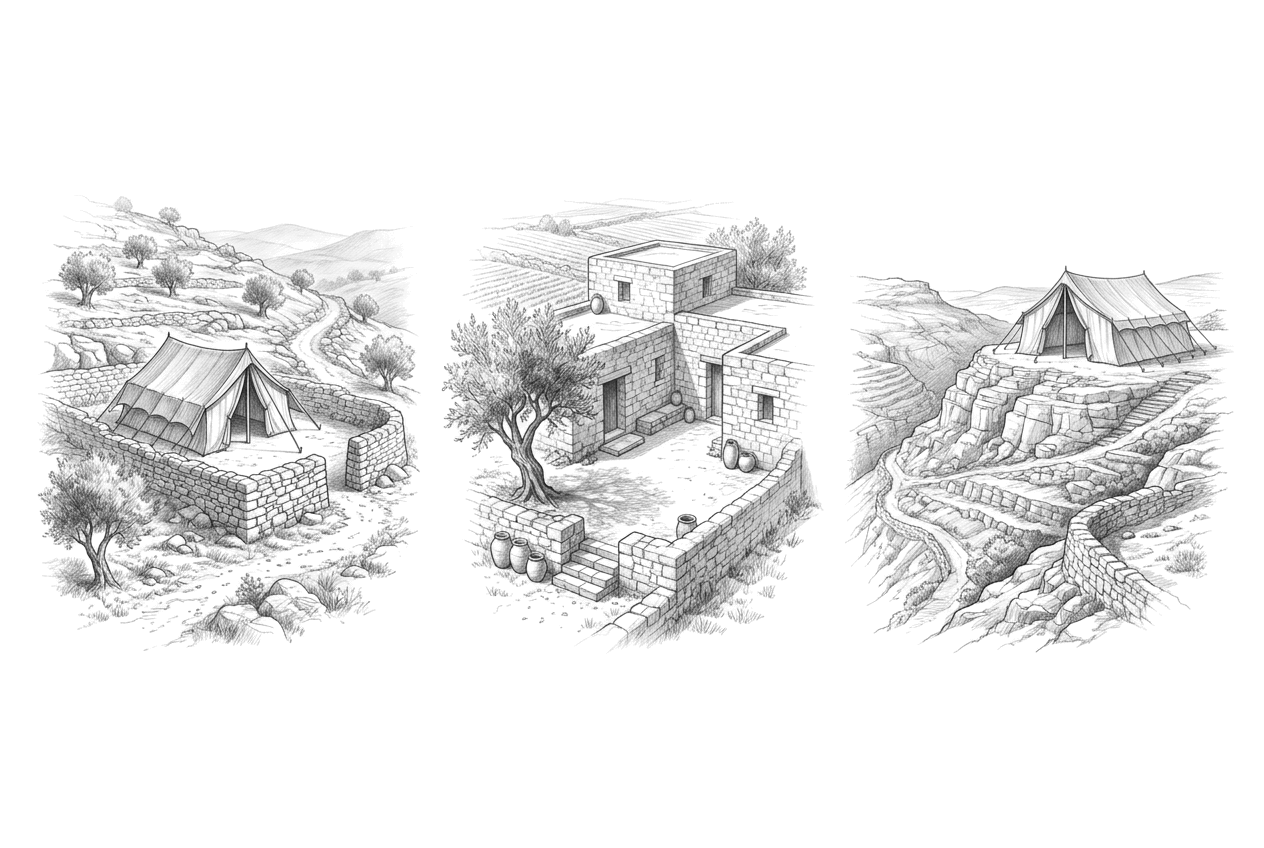
\includegraphics[width=0.95\linewidth]{theology/mariology/ark-of-the-covenant/artwork/shiloh-kiriath-david-graphite.png}%
  };
  \begin{scope}[x={(image.south east)}, y={(image.north west)}]
    \node[anchor=center, align=center, font=\scriptsize, text width=0.31\linewidth] at (0.175, 0.115) {%
      \textbf{I. Shiloh}\\[-0.05em]\textit{Highland sanctuary\\(Jos 18:1; 1 Sam 1--4)}%
    };
    \node[anchor=center, align=center, font=\scriptsize, text width=0.31\linewidth] at (0.50, 0.115) {%
      \textbf{II. House of Obed-edom}\\[-0.05em]\textit{Three months of blessing\\(2 Sam 6:10--12)}%
    };
    \node[anchor=center, align=center, font=\scriptsize, text width=0.31\linewidth] at (0.825, 0.115) {%
      \textbf{III. Tent on Mount Zion}\\[-0.05em]\textit{Royal dwelling prepared\\by David (2 Sam 6:17)}%
    };
  \end{scope}
\end{tikzpicture}
\end{center}\nopagebreak[4]
\else
\begin{studybox}{Plate III: Three Sanctuaries on the Road to Zion}
Three monochrome vignettes trace the Ark's resting places from the era of the Judges to the kingdom of David:
\begin{itemize}
  \item \textbf{I. Shiloh (Jos 18:1; 1 Sam 1--4):} A pitched sanctuary tent framed by a low fieldstone enclosure upon terraced olive-bearing hills in Ephraim, recalling the long-settled shrine where Samuel ministered before the lamp of God went out and from which Israel rashly bore the Ark into battle.
  \item \textbf{II. House of Obed-edom (2 Sam 6:10--12; 1 Chr 13:14):} A modest stone courtyard dwelling shaded by an olive tree and ringed with household storage jars, illustrating the quiet domestic shelter in Judah where the Ark remained three months and poured blessing upon Obed-edom and all his household.
  \item \textbf{III. Tent on Mount Zion (2 Sam 6:17; 1 Chr 16:1):} A royal pavilion pitched high atop a steep limestone ridge reached by a stepped mountain ascent, depicting the prepared sanctuary in the city of David where the Levites set the Ark amid joyful shouting, sacrifice, and perpetual praise.
\end{itemize}
\end{studybox}
\fi

\begin{platecaption}
\textbf{Plate III. Three resting places between the conquest and the Temple.} From left to right: the highland sanctuary at Shiloh (Jos 18:1; 1 Sam 1--4), the Judean household of Obed-edom where the Ark remained three months in blessing (2 Sam 6:10--12; 1 Chr 13:14), and the tent David pitched for the Ark upon Mount Zion (2 Sam 6:17). Because the exact architectural forms of Shiloh's shrine, Obed-edom's dwelling, and David's tent are unrecovered, these vignettes offer disciplined visual orientation rather than archaeological reconstruction.
\end{platecaption}
